% * осмыслить и подредактировать
% * добавить графику
\chapter{Введение}

Разработкой видеоигр занимается разработчик, который может быть представлен как одним человеком, так и
фирмой. Обычно крупномасштабные коммерческие игры разрабатываются командами разработчиков в пределах
компании, специализирующейся на играх для персонального компьютера или консолей. Как правило, разработку
финансирует другая, более крупная компания-издатель, которая по окончании разработки занимается изданием
игры и связанными с ним тратами. Реже компании-издатели могут содержать внутренние команды разработчиков,
или же компания-разработчик может разрабатывать игры за свой счет и распространять их без участия издателей,
например, средствами цифровой дистрибуции (инди-игры).

Разработка наиболее крупнобюджетных игр (<<AAA-игры>>) может стоить десятки миллионов долларов США, причем в
течение последних десятилетий эти бюджеты непрерывно росли, как и численность команд разработчиков и сроки
разработки. Так, в конце девяностых игру для консоли PlayStation в верхнем ценовом сегменте -- 60 долларов
США для конечного покупателя -- могла сделать команда из 10 человек за год, для PlayStation 2 (первая
половина 2000-х) необходима была команда из 30-50 человек и два года разработки, к 2012 году речь шла уже
о командах из свыше чем 100 разработчиков и срок порядка трех лет. По утверждению Алекса Мура, геймдизайнера
из компании Sumo Digital, если бы цена игры для конечного потребителя росла в той же пропорции, игры в 2012
году стоили бы по 1800 долларов США; иными словами, чтобы окупить возросшие бюджеты при сохранении тех же
цен в магазинах, компании-издатели должны продавать намного больше копий игр \cite{1.1}.

Средний бюджет ААА-проекта -- как правило, речь о играх, выпускаемых крупнейшими компаниями-издателями,
продающихся на физических носителях и нередко входящих в состав известной серии из нескольких игр --
колеблется от 18 до 24 млн долл. Если речь идёт о продукте для одной единственной платформы, то его
стоимость составит около 10 млн долл\cite{1.2}. Крупнобюджетная игра для двух платформ -- Xbox 360 и
PlayStation 3 -- обходилась в 2012 году в среднем в 20 миллионов долларов, и для того, чтобы она окупилась,
нужно было продать около двух миллионов копий\cite{1.3}.

Для российских компаний разработка среднего проекта обходится в среднем от 100 тысяч до миллиона долларов.
Стоимость разработки маленьких российских проектов идет от 10 тысяч долларов\cite{1.4}. Разработку обычно
финансирует издатель, хотя последнее время появляются успешные примеры финансовых вливаний из индустрий,
не связанных с геймдевом \cite{1.6}. Процесс разработки обычной современной игры занимает около года, 
для АААпроектов может затянуться до 2-3 лет, цикл разработки <<казуальных>> игр занимает порядка 4-6 
месяцев, притом, что идет конвейерная разработка сразу 2-3 проектов.

\chapter{Классификация компьютерных игр}
Прежде чем рассматривать процесс разраработки давайте сначал произведём классификацию игр. Компьютерные 
игры в основном классифицируются по жанрам, а также по количеству игроков. Вследствие того, что критерии 
принадлежности игры к тому или иному жанру не определены однозначно, классификация компьютерных игр 
недостаточно систематизирована, и в разных источниках данные о жанре конкретного проекта могут различаться. 
Один из примеров классификации представлен на рисунке (\ref{img:genre}). Тем не менее, существует 
консенсус, к которому пришли разработчики игр, и принадлежность игры к одному из основных жанров почти 
всегда можно определить однозначно. Наиболее популярные жанры (в которых можно выделить множество 
поджанров) перечислены ниже.

\begin{figure}[!ht]
    \center
    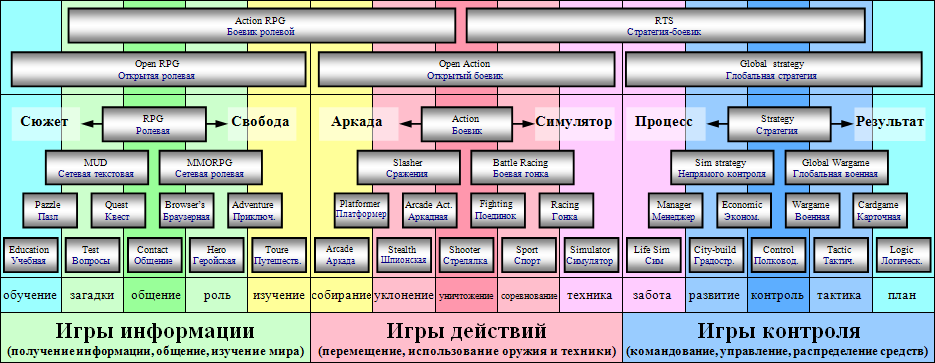
\includegraphics[width=1.0\textwidth]{genre}
    \caption{Классификация жанров компьютерных игр\cite{genre}}
    \label{img:genre}
\end{figure}

\emph{Action}. Действие таких игр развивается очень динамично и требует напряжения внимания и быстрой 
реакции на происходящие в игре события. При этом в качестве основного средства прогресса в игре, как 
правило, используется какое-либо оружие. \emph{Представители:} Space Invaders, 
серия Uncharted (рис.~\ref{img:uncharted}), Doom. \\

\emph{3D Shooter}. В играх данного типа игрок, как правило, действуя в одиночку, должен уничтожать 
врагов при помощи оружия ближнего боя и стрелкового оружия, для достижения определённых целей на 
данном уровне, обычно, после достижения заданных целей игрок, переходит на следующий уровень. 
\emph{Представители:} Duke Nukem 3D, System Shock, Half-Life.\\

\emph{FPS и TPS}. В шутерах от первого лица (FPS) игрок не видит персонажа со стороны -- он наблюдает 
за происходящим от лица персонажа -- <<глазами персонажа>>, и наблюдаемая игроком картина совпадает 
с тем, что <<видит>> персонаж. В шутерах от третьего лица (TPS) игрок видит персонаж со стороны с 
фиксированной или произвольной точки зрения. В ряде игр реализована возможность переключения 
первое/третье лицо и фиксированная/произвольная камера. \emph{Представители:} Doom, Quake, 
Unreal Tournament, Tomb Raider, Max Payne, Grand Theft Auto. \\

\emph{Tactical Shooter}. Принципиальное отличие тактических шутеров от классических состоит в том, 
что персонаж не изображает героя-одиночку, а действует в составе команды. В тактическом шутере обычно 
воссоздаётся деятельность отрядов -- взаимодействие между бойцами, маневрирование и выбор направления 
атаки, подбор команды и её вооружения. В одиночном режиме эти возможности реализуются ботами, в 
сетевом -- через взаимодействие живых игроков. \emph{Представители:} Battlefield, Counter-Strike, 
Delta Force.

\begin{figure}[!ht]
    \centering
    \begin{subfigure}[b]{0.45\textwidth}
        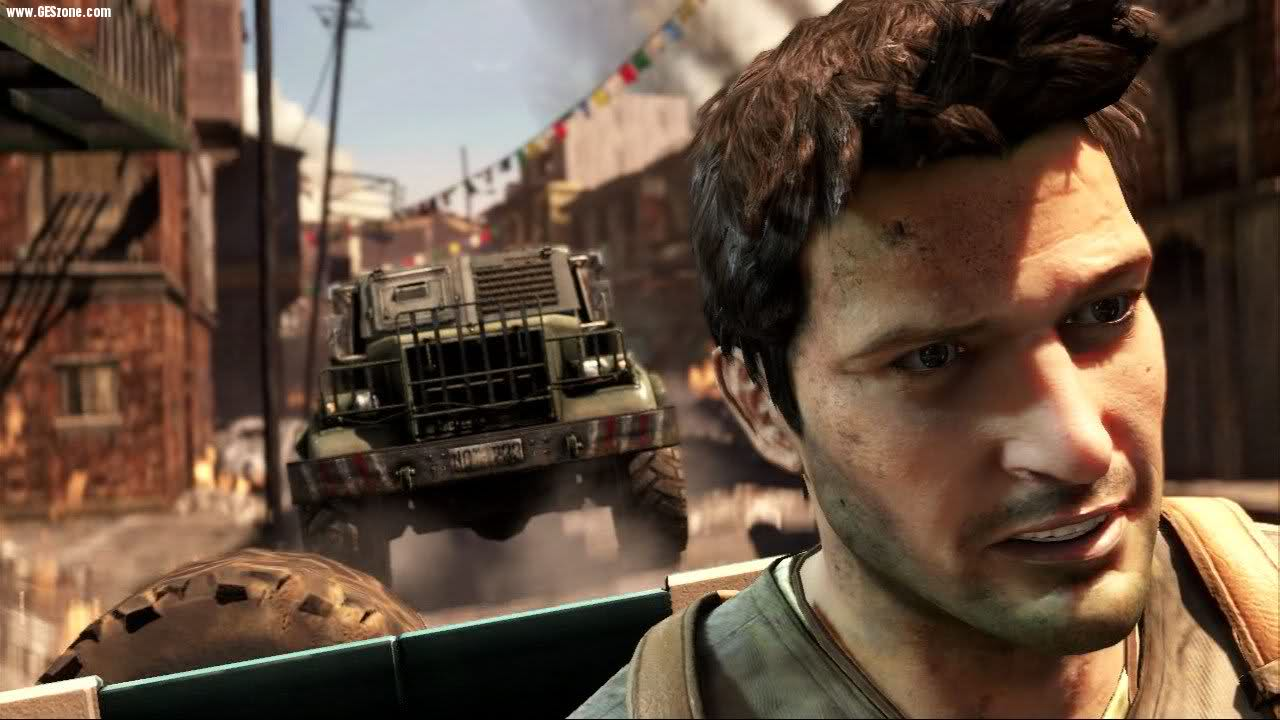
\includegraphics[width=\textwidth]{action_game}
        \caption{Uncharted}
        \label{img:uncharted}
    \end{subfigure}
    \begin{subfigure}[b]{0.45\textwidth}
        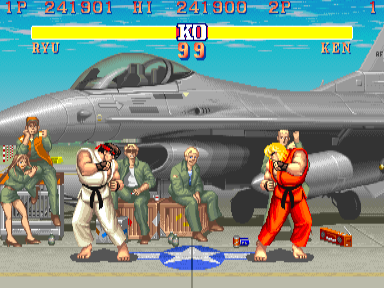
\includegraphics[width=\textwidth]{fighting_game}
        \caption{Street Fighter IV}
        \label{img:street}
    \end{subfigure}
    \caption{Игры жанров Action и Fighting}
\end{figure}

\emph{Fighting}. Геймплей состоит исключительно из поединков двух и более противников с применением 
рукопашного боя. \emph{Представители:} Mortal Kombat, Street Fighter (рис.~\ref{img:street}), 
Tekken.\\

\emph{Beat ’em up}. Разновидность файтингов, бой в которых происходит за пределами арены и со 
множеством противников одновременно. \emph{Представители:} Battletoads, Comix Zone, 
Enter the Matrix.\\

\emph{Hack and Slash}. Игры с видом от третьего лица, основной частью игрового процесса, в которых 
являются фехтовальные поединки с применением холодного и другого оружия. \emph{Представители:} 
Devil May Cry (рис.~\ref{img:dmc}), Torchlight, Diablo.\\

\emph{Arcade}. Игра, в которой игроку приходится действовать быстро, полагаясь в первую очередь на свои 
рефлексы и реакцию. Игровой процесс прост и не меняется в течение игры. Аркады характеризуются 
развитой системой бонусов: начисление очков, постепенно открываемые элементы игры и т. д. 
\emph{Представители:} Battle City, Mega Man (рис.~\ref{img:mega}), Super Mario Bros.\\

\emph{Stealth-action}. Игры, в которых предполагается не сражаться с большинством встреченных 
противников, а всячески избегать возможного контакта с ними, попутно выполняя поставленные задачи. 
\emph{Представители:} Metal Gear Solid, Tom Clancy's Splinter Cell, Dishonored. \\

\begin{figure}[!ht]
    \centering
    \begin{subfigure}[b]{0.45\textwidth}
        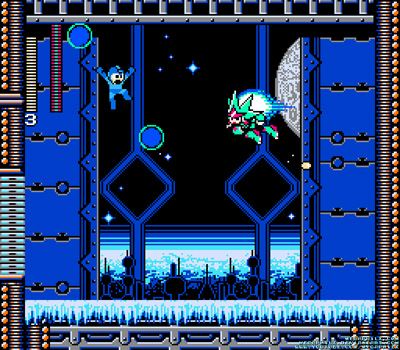
\includegraphics[width=\textwidth]{arcade_game}
        \caption{Mega Man}
        \label{img:mega}
    \end{subfigure}
    \begin{subfigure}[b]{0.45\textwidth}
        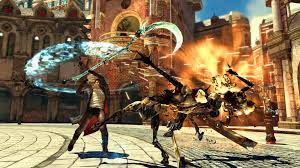
\includegraphics[width=\textwidth]{slash_game}
        \caption{Devil May Cry}
        \label{img:dmc}
    \end{subfigure}
    \caption{Игры жанров Arcade и Hack and Slash}
\end{figure}

\emph{Simulator}. Игры, предоставляющие возможность симуляции и управления тем или иным процессом 
из реальной жизни. \emph{Представители:} Ил-2 Штурмовик, Need for Speed, FIFA. \\

\emph{RTS и TBS}. Игры, требующие планирования и выработки определенной стратегии для достижения 
некоей конкретной цели, например, победы в военной операции. Игрок управляет не одним персонажем, а 
целым подразделением, предприятием или даже вселенной. Различают походовые или пошаговые 
стратегические игры (TBS), где игроки поочерёдно делают ходы, и каждому игроку отводится 
неограниченное или ограниченное время на свой ход, и стратегические игры в реальном времени (RTS), 
в которых все игроки выполняют свои действия одновременно, и ход времени не прерывается. 
\emph{Представители:} серия Command \& Conquer (рис.~\ref{img:cnc}), Civilization, 
Hearthstone: Heroes of Warcraft.\\

\emph{Adventure}. Игра-повествование, в которой управляемый игроком герой продвигается по сюжету 
и взаимодействует с игровым миром посредством применения предметов, общения с другими персонажами 
и решения логических задач. \emph{Представители:} Space Quest, Monkey Island, Deponia, Machinarium.\\

\begin{figure}[!ht]
    \centering
    \begin{subfigure}[b]{0.45\textwidth}
        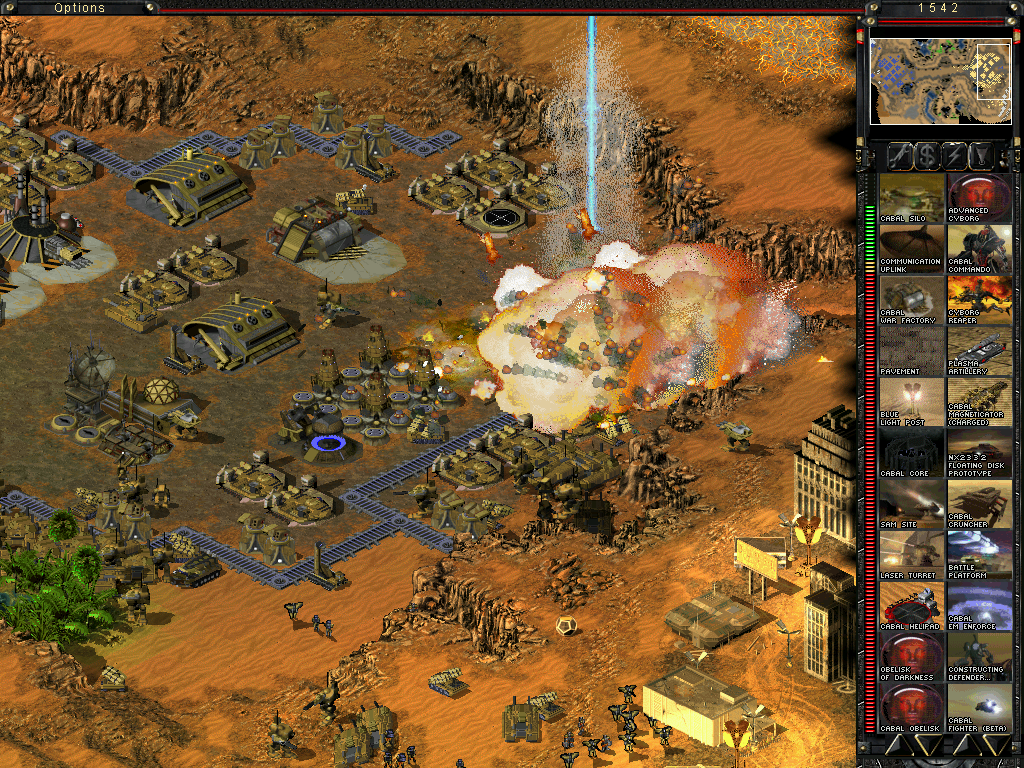
\includegraphics[width=\textwidth]{rts_game}
        \caption{C\&C: Tiberian Sun}
        \label{img:cnc}
    \end{subfigure}
    \begin{subfigure}[b]{0.45\textwidth}
        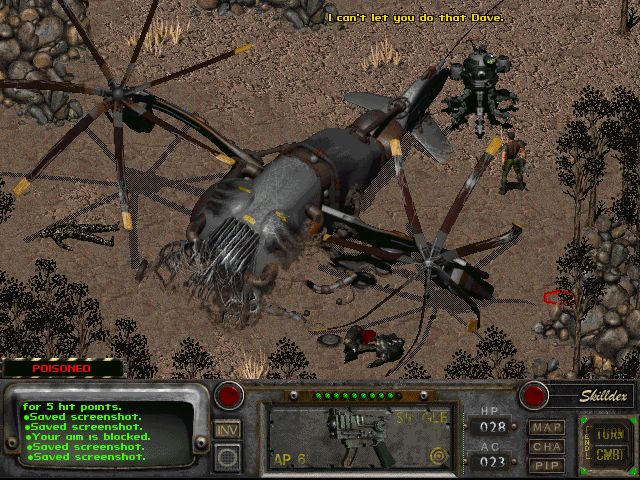
\includegraphics[width=\textwidth]{rpg_game}
        \caption{Fallout 2}
        \label{img:fallout}
    \end{subfigure}
    \caption{Игры жанров RTS и RPG}
\end{figure}

\emph{Rhythm game}. В музыкальных играх геймплей строится на взаимодействие игрока с музыкой. Жанр 
же может быть любой, от головоломок до ритм игр. \emph{Представители:} Guitar Hero, Rock Band, 
Frets on Fire. \\

\emph{RPG}. Жанр компьютерных игр, основанный на элементах игрового процесса традиционных настольных 
ролевых игр. В ролевой игре игрок управляет одним или несколькими персонажами, каждый из которых 
описан набором численных характеристик, списком способностей и умений; примерами таких характеристик 
могут быть хит-поинты (HP), показатели силы, ловкости, защиты, уклонения, уровень развития того или 
иного навыка и т.п. В ходе игры они могут меняться. Одним из характерных элементов игрового процесса 
является повышение возможностей персонажей за счёт улучшения их параметров и изучения новых 
способностей. \emph{Представители:} серия Fallout (рис.~\ref{img:fallout}), серия The Elder Scrolls, 
серия Mass Effect.

\emph{Puzzle}. Название жанра компьютерных игр, целью которых является решение логических задач, 
требующих от игрока задействования логики, стратегии и интуиции или в иных случаях некоторого наличия 
удачи. \emph{Представители:} The Lost Vikings, Sokoban, Portal.\\

\emph{Traditional}. Компьютерная реализация настольных игр. \emph{Представители:} карты, шахматы, 
монополия.\\

\emph{Interactive fiction}. Жанр компьютерных игр, в котором общение с игроком осуществляется посредством 
текстовой информации. Развитие этого жанра, в связи с низким требованием к ресурсам, началось весьма 
давно, и не прекратилось даже с появлением графических игр.
\emph{Представители:} Colossal Cave Adventure, Photopia, Façade.

\chapter{Специализации}
В начале 1980-х, в раннюю эпоху домашних компьютеров и игровых приставок, единственный игровой программист
мог управлять почти всеми задачами разработки игры. Однако разработка современных коммерческих видеоигр
предполагает наличие широкого круга навыков и персонала поддержки. Как результат, для работы над одним
проектом часто требуются целые команды. В состав типичной современной команды разработчиков обычно входят
представители разных специализаций.

\section{Разработчики графического контента и ассетов}
\begin{itemize}
    \item \emph{Арт-директор.} Как правило, это наиболее опытный и уважаемый член команды из занимавшихся
        созданием контента. Его задачей является контроль качества и времени исполнения.
    \item \emph{2D-художник.} Основная задача 2D-художников состоит в создании двухмерных персонажей для
        соответствующих игр (флеш-игры, некоторые браузерные игры, игры для социальных сетей и т. д.). Также
        их работы используются в рекламных и маркетинговых компаниях, при создании сайта игры для
        взаимодействия с игровым сообществом, для наполнения установщика игры, позволяя им по мере набора
        опыта становиться или концепт-художником, или дизайнером интерфейса, или 2D-художником в
        нетрёхмерном проекте, или художником по текстурам.
    \item \emph{Концепт-художник.} Его задачей является отправить чёрно-белые и, возможно, впоследствии
        раскрашенные наброски на утверждение арт-директору, продюсеру, инвесторам, директорату или службе
        контроля качества лицензиата сеттинга, чтобы впоследствии донести их идеи и виденье игры до всех
        остальных художников проекта.
    \item \emph{Художник по текстурам} -- очередная специализация 2D-художника, который способен создать
        текстуру для 3D-модели в соответствии с концептом.
    \item \emph{3D-художник.} В его задачи входят: создание 3D-сетки моделей зданий и техники в
        специализированных программах, как то: LightWave, 3D Studio Max, Autodesk Maya, Blender и др.
    \item \emph{3D-Художник персонажей.} 2 узкоспециализированных подкласса 3D-художников, создающих
        высокополигональные модели разного рода органики. Зачастую, для уменьшения нагрузки на платформу
        игры (особенно если платформой является ПК) используется технология так называемого рельефного
        текстурирования (bump mapping), при которой высокая детализация достигается наложением текстуры
        рельефа, а не изменением самой модели.
    \item \emph{Аниматор или mocap studio.} более старым методом создания движения является key framing,
        который до сих пор используется для анимирования негуманоидных монстров, техники, и нереальных для
        исполнения живым актёром движений. mocap является более современным методом, дающим более плавную и
        реалистичную картину движения гуманоидного персонажа.
    \item Художник спецэффектов.
\end{itemize}

\section{Дизайн}
\begin{itemize}
    \item \emph{Ведущий дизайнер} -- помимо генерации и развития основной идеи, его задачей является
        координация работы остальных дизайнеров. Его работа построена на тесном взаимодействии с арт
        директором и ведущим программистом и заключается не только в добавлении идей в игру, но и в
        определении того, что стоит в неё вносить. Помимо этого он выполняет задачи, с которыми не в
        состоянии справиться дизайнерская команда.
    \item \emph{Дизайнер игровой механики.} Как правило он в прошлом был программистом и представляет как
        идеи превращаются в код. В задачу дизайнера по механике входит, получив идею от ведущего дизайнера,
        пообщавшись с дизайнером миссий или уровней, составить список требований программистам. А дальше
        многократно проигрывая отдельные фрагменты игры, получить представление, насколько их понимание
        игровой механики сбалансировано.
    \item \emph{Дизайнер миссий или уровней.} Им может быть скриптовик, пишущий код для встроенного в игру
        интерпретатора, или художник, создающий игровую карту в редакторе уровней, или кто-то ещё, просто
        описывающий на формальном языке, из чего должен состоять уровень.
    \item \emph{Дизайнер UI} разрабатывает функционал пользовательского интерфейса, иногда собирает его из
        контента предоставленного художниками с помощью инструментов, сделанных программистами.
    \item \emph{Сценарист} -- в отличие от писателя или сценариста в кино его повествование должно быть
        интерактивным и, как следствие, он должен постоянно обсуждать дальнейшее развитие сюжета с
        дизайнерами, чтобы определить, что возможно сделать на скриптовом языке, в редакторе карт и иных
        утилитах. Как и коллеги по литературе и кино, он должен владеть родной речью и литературным языком,
        этот талант сродни музыкальному слуху, позволяет тону и словам, произносимым игровыми персонажами,
        звучать реалистично.
\end{itemize}

\section{Звук}
\begin{itemize}
    \item \emph{Инженер по звуковым эффектам} -- ищет нужный звук в библиотеке, либо записывает новый с
        натуры, либо синтезирует подходящий из одного и более существующих
    \item \emph{Композитор} -- создаёт или синтезирует музыкальное оформление для игры
    \item \emph{актёры озвучивания} -- озвучивают персонажей
\end{itemize}

\section{Контроль качества}

Единственный способ убедиться в качестве игры -- это поиграть в неё, в небольших компаниях на начальных
стадиях за качество отвечает линейный продюсер, в более крупных проектах обосабливаются следующие команды:
\begin{itemize}
    \item \emph{QA (контроль качества) команда издателя} -- как и все отслеживают дефекты в контенте и баги,
        как правило указывая при этом какие баги править в первую очередь, наиболее жёстко из всех следят
        за тем, чтобы разработка укладывалась в график
    \item \emph{QA основная} -- внутренняя команда разработчика, оценивает одиночный режим игры
    \item \emph{QA мультиплеер} -- если игра будет позиционироваться как мультиплеерная, то создаётся
        отдельная команда, которая им занимается
    \item \emph{QA внешняя} -- чтобы получить независимый взгляд, иногда оплачиваются услуги
        профессиональных тестировщиков аутсорсеров, т.к. они не участвовали в разработке, у них лучше
        получается выявлять баги в кривой обучения игрока
    \item \emph{QA совместимости} -- если игру помимо консолей планируется выпустить на ПК, её гоняют на
        нескольких десятках самых различных конфигураций; проверяется правильность настроек
        производительности и поддержка основной массы <<железа>>
    \item \emph{QA локализации} -- проверяется качество перевода
    \item \emph{бета-тестеры} -- это неоплачиваемые фанаты будущей игры, которые захвачены идеей её улучшить
        ещё до релиза, в случае откровенно слабого тайтла издатель может принять решения об отмене
        бета-тестирования, т.к. помимо того, что оно в любом случае удлиняет сроки разработки, в данном
        случае оно ещё и не позволяет <<продавить>> рынок под эту игру увеличением маркетингового бюджета.
        Единственным исключением здесь являются массивные многопользовательские игры, которые в силу
        специфики их монетизации в любом случае выигрывают от бета-тестирования
    \item \emph{управляющий бета-тестированием} -- как правило это линейный продюсер или сопродюсер,
        которому достаётся наиболее стрессовая часть общения с фанатами, которые обычно очень эмоционально
        описывают баги и требуют новые фичи.
\end{itemize}

\section{Программирование}
\begin{itemize}
    \item \emph{ведущий программист} -- до 90-х гг мог быть единственным программистом, как правило, это
        программист с наибольшим опытом, и не обязательно руководитель, т. к. иногда управление кодингом
        перекладывается на технического директора, которому отчитываются руководители отделов
    \item \emph{технический директор} -- в крупных компаниях отвечает за качество кода и архитектурных
        решений (соблюдение стандартов, возможность повторного использования и т. д.) сразу на нескольких
        проектах
    \item \emph{программист игровой механики} -- именно от него зависит, как игрок и сущности
        взаимодействуют друг с другом, будь то удар меча по ящику или выстрел пушки, раскидывающий всех по
        округе
    \item \emph{3D-программист} -- от него зависит отображение мира на экране, поэтому от него требуются
        глубокие познания в векторной алгебре, численных методах, тригонометрии
    \item \emph{программист AI} -- требования к нему сильно размыты при переходе от одного к другому
        жанру; именно он предоставляет возможность дизайнеру уровней задавать через триггеры и скрипты
        ответ окружения, мобов, NPC на действия игрока
    \item \emph{программист UI} -- создаёт пользовательский интерфейс, позволяющий данным с HUD
        воздействовать на игровую механику, будь то выбор меню или осмотр карты
    \item \emph{программист инструментов (утилит)}, в т. ч. редактора уровней -- наиболее трудоёмкая
        должность, но именно он экономит основную часть времени художников и дизайнеров, делая более
        производительные редакторы моделей, уровней, триггеров, игровых параметров и прочего контента
    \item \emph{программист сетевого кода} -- создаёт сетевой движок игры для поддержки мультиплеера,
        кооператива, скачивания обновлений и т.д.
\end{itemize}

\section{Управление}
\begin{itemize}
    \item \emph{линейный продюсер} -- решает повседневные вопросы компании, начиная от заказа ужина для
        заработавшихся работников и прохладительных напитков в жаркий день, заканчивая рассылкой свежих
        билдов бета-тестировщикам и издателю, следит за тем, чтобы разработчики не слишком много рабочего
        времени уделяли <<изучению>> продукции конкурентов
    \item \emph{сопродюсер (associate)} -- как следует из названия, объединяет работу нескольких команд
        или офисов, отвечает за обновление и доведение планов до участников команды, отчитывается за их
        выполнение перед начальством
    \item \emph{исполнительный продюсер} -- отвечает за составление планов и их своевременное исполнение в
        контексте бюджета, ведёт переговоры с инвесторами, издателями, заключает сделки со сторонними
        разработчиками, решает кадровые вопросы
\end{itemize}

\section{Другие специальности}
При разработке ММО возникает необходимость в поддержке проекта, что влечёт за собой появление дополнительных
специальностей -- операторский отдел, платёжный отдел (и создание платёжной системы), гейм-мастера, отдел
продаж, рекламный и т. д.

Некоторые члены команды могут выполнять несколько функций. Например, продюсер также может быть дизайнером
или ведущим программистом. Однако, если в начале эпохи видеоигр это было обычным явлением, то сейчас, при
разработке профессиональных игр, это встречается всё реже и реже.

\chapter{Процесс разработки}
Процесс разработки игры меняется в зависимости от компании и проекта. Однако разработка коммерческой игры
обычно включает следующие этапы:

\section{Предпроизводственный процесс}
Ранние стадии разработки игры часто характеризуются низким качеством графики. Особенно это справедливо для
различных игровых прототипов.

Обычно перед началом разработки любой игры должна сформироваться идея, а издатель/разработчик должен дать
<<зелёный свет>>.

В более распространённом случае, если разработчик и издатель являются разными компаниями, идея должна быть
предложена руководству, одобрена и выставлена на рассмотрение издателям. В этом деле может помочь рабочее
демо, но оно не является обязательным для авторитетного издателя с хорошей репутацией. Если заинтересованный
издатель найден, можно начинать производство. Сегодня идея игры редко убеждает, если в ней не заинтересован 
издатель.

Если разработчик также является издателем, или если они оба являются подразделениями одной компании, то
добрение должно дать только высшее руководство. Однако, в зависимости от размера компании-издателя, может
потребоваться несколько попыток, пока идея не поднимется вверх через все слои руководства.

Представителем проекта обычно является геймдизайнер, но им также может быть человек из игровой индустрии
любой другой должности. Перед началом полномасштабного производства геймдизайнер должен написать
дизайн-документ -- подробный документ, описывающий концепцию и геймплей. Также он может содержать некоторые
предварительные скетчи различных аспектов игры. Некоторые геймдизайнеры включают в дизайн-документ даже
примерный рабочий прототип, демонстрирующий одну или несколько сторон игры. Обычно дизайн-документ
объединяет в себе все или большую часть материалов начального замысла. Основная особенность
дизайн-документа -- это его <<живость>> -- в действительности он не будет завершён до тех пор, пока игра
находится в разработке. Он может изменяться каждую неделю, иногда -- каждый день. Поэтому, даже если
дизайн-документ должен существовать в некоторой форме перед началом полномасштабного производства, он почти
никогда не является завершённым дизайном, хотя может описывать многие аспекты всех стадий полностью
спроектированной игры.\cite{main}

Перед тем, как появится одобренный дизайн, основная команда программистов и художников может начать работу
над идеями. Программисты могут разработать начальные прототипы для демонстрации одной или нескольких
возможностей, которые хотят видеть в игре некоторые посредники. Или они могут начать разработку каркаса,
который, в конечном счёте, будет использоваться игрой. Художники могут нарисовать эскизы, как плацдарм для
разработки реальных игровых ресурсов. Сначала продюсер может работать над игрой неполный рабочий день, но 
повышать свою занятость по мере продвижения разработки.

\section{Производство}
На этапе основного производства выполняется огромный объём работ. Программисты пишут исходный код, художники
рисуют графику (спрайты или 3D-модели игровых элементов). Звукооператоры разрабатывают звуковые эффекты, а
композиторы пишут музыку для игры. Дизайнеры уровней создают уровни, а писатели пишут диалоги для скриптовых
сцен и неигровых персонажей.

Всё это время геймдизайнер дополняет и изменяет игровой дизайн, чтобы отразить текущее видение игры.
Некоторые особенности или уровни могут быть удалены, некоторые добавлены. Художественная трактовка может
эволюционировать, а сюжет (предыстория) -- измениться. Может появиться новая целевая платформа, а также
новая целевая аудитория. Все эти изменения должны быть задокументированы и большинство из них должно
появиться в дизайн-документе.

С точки зрения времени, первый уровень игры разрабатывается дольше всех остальных. Поскольку дизайнеры
уровней и художники используют инструменты для создания уровней, им требуются возможности и изменения
внутренних инструментов. С появлением новых возможностей некоторые уровни могут устареть, поэтому, в первый
уровень игры могут вноситься различные исправления. Кроме того, в силу динамической природы разработки игр,
дизайнерское видение первого уровня с течением времени может изменяться. Довольно обычным является потратить
на первый уровень более 12 месяцев при общей трёхлетней разработке игры. Последующие уровни могут
разрабатываться значительно быстрее, так как список возможностей становится более полным, а видение
игры -- более ясным.

Тестеры подключаются к игре, когда появляется что-то играбельное. Это может быть один уровень или
подмножество игры, которое может использоваться в любых разумных пределах. На раннем этапе тестирование
игры отнимает у одного тестера относительно малую долю времени; в любое время тестеры могут быть
ответственны сразу за несколько игр. По мере приближения разработки к концу, одна игра может начать отнимать
у тестеров всё их время -- и даже сверхурочно -- поскольку они стараются протестировать новые возможности,
для которых существуют тесты регрессии. Сегодня тестирование является жизненно важным для игр, поскольку, в
силу сложности большинства из них, одно-единственное изменение может привести к катастрофическим
последствиям.\cite{main}

\section{Поддержка}
В обычном случае поддержка заключается в выпуске патчей для исправления ошибок, найденных уже после выхода
игры. Однако, в случае ММО, поддержка может сравняться или даже превосходить производство как по
трудоёмкости, так и по времени, так как успешная ММО должна непрерывно развиваться и расширяться, чтобы
избежать оттока игроков.

\section{Аутсорсинг}
Некоторые аспекты производства видеоигр, такие как создание и подбор музыки и звуков, актёрская озвучка или
захват движения, зачастую требуют крупных и не всегда целесообразных финансовых вложений, если выполнять их
силами самого разработчика (это может быть эффективным только в том случае, если разработчик создаёт
несколько игр одновременно и имеет внутренние отделы для реализации конкретных задач). Нанимать сотрудников
в штат для выполнения этих задач компаниям не выгодно, поэтому абсолютное большинство разработчиков
прибегают к услугам соисполнителей для выполнения части своего проекта -- отдают их на аутсорсинг
\cite{1.8,1.9}.

Планы касательно аутсорсинга рассматривают на этапе подготовки производства; именно тогда рассчитывают
необходимые временные и финансовые затраты на работу, которая будет произведена вне компании-разработчика.
\begin{itemize}
    \item Программирование обычно не отдают на аутсорсинг. Однако, некоторые модульные инструменты, такие
        как видео-компрессор или редактор уровней могут быть отданы другой студии на разработку.
    \item Цены на создание музыкальных треков разнятся в стоимости в зависимости от длины, метода
        произведения (синтез или живое исполнение) и опыта композитора. В 2003 г. минута высококачественной
        синтезированной музыки стоила \$600-1500; 60 минут музыки для игры с 20 часами геймплея могли
        обойтись издателю в 50-60 тыс. долларов\cite{1.11}.
    \item Актёрская озвучка как аспект производства хорошо подходит для аутсорсинга, т.к. требует набор
        конкретных узкоспециальных навыков. Лишь наиболее крупные издатели принимают актёров озвучивания в
        штат.
    \item Студии для захвата движения (motion capture) очень дороги и сложны в постройке, поэтому небольшим
        компаниям нецелесообразно иметь собственные студии для захвата движения, гораздо выгоднее 
        воспользоваться услугами компаний-аутсорсеров.
\end{itemize}

\chapter{Инди-игры}
Инди-игры (англ. Indie games, от англ. independent video games -- <<независимые компьютерные игры>>) -- это
компьютерные игры, созданные отдельными разработчиками или небольшими коллективами без финансовой поддержки
издателя компьютерных игр. Распространение осуществляется посредством каналов цифровой дистрибуции. Масштаб
явлений, связанных с инди-играми, ощутимо возрастает со второй половины 2000х годов, в основном ввиду
развития новых способов онлайн-дистрибуции и средств разработки.

Некоторые инди-игры добились значительной популярности, например, Braid\cite{2.1}, World of Goo\cite{2.2}, 
The Path, Papers, Please или Minecraft\cite{2.3}

\section{Общее описание}
Общепринятого определения понятия <<инди-игра>> не существует\cite{2.5,2.7}. Но, зачастую, 
инди-игры имеютнекоторые схожие особенности. Инди-игры создаются отдельными разработчиками, небольшими 
коллективами или маленькими независимыми компаниями\cite{2.5}. Также инди-игры обычно не такие 
масштабные, как массовые игры с полным финансированием. Разработчики инди-игр, как правило, не 
имеют финансовой поддержки от издателя (так как они предпочитают наименее рисковые игры с высоким 
бюджетом\cite{2.10}), и обычно обладают небольшим бюджетом, либо не обладают им вовсе
\cite{2.5,2.7,2.12}. Ввиду своей независимости инди-разработчики не имеют операционных 
ограничений со стороны издателей или творческих ограничений\cite{2.5,2.13,2.7} и не нуждаются в
одобрении издателя, что является обязательным для разработчиков массовых игр. Как 
следствие, решения геймдизайнера также не ограничиваются бюджетом проекта\cite{2.13}. Более того, чем меньше 
коллектив, тем ярче выражается индивидуальность конкретного разработчика\cite{2.15}. Небольшие коллективы, 
широкие возможности и отсутствие границ для творчества создали условия, в которых инди-игры могут быть 
инновационными, креативными, с большим художественным выражением\cite{2.15,2.16,2.17,2.19}. 
Ограниченные в возможностях создания технологичной графики, разработчики вынуждены делать ставку на 
инновационный геймплей\cite{2.20}. Впрочем, среди инди-игр существуют как инновационные игры, так и игры 
классических жанров\cite{2.17}. Таким образом, принадлежность к <<инди>> не подразумевает, что игра должна 
нести в себе инновации\cite{2.21}.

\section{Разработка}
В поисках источника финансирования новой игры инди-разработчики могут прибегать к краудфандингу, поиску
издателя\cite{2.12,2.22,2.23} или создания помогающего сообщества в течение разработки игры\cite{2.24}. 
Если у проекта нет издателя, разработчики используют предлагаемые в интернете службы цифровой 
дистрибуции. Большинство инди-игр не приносит существенного дохода\cite{2.26}.

Разработчиков инди-игр не следует путать с разработчиками-любителями, для которых это занятие является
хобби, поскольку инди-разработчики сильнее нацелены на выпуск продукта, нежели любители. 
Большинство любителей создает модификации к существующим компьютерным играм, либо работает с 
некоторыми технологиями или определенными частями игры. Подобные любители обычно создают 
некоммерческие продукты, и сами по себе могут быть как новичками, так и ветеранами индустрии.

\section{Положение в индустрии}
Сцена инди-игр зародилась на ПК\cite{2.5}, где продолжает оставаться заметной\cite{2.19}. В начале 1990х 
годов инди-игры испытали первую волну популярности благодаря модели распространения shareware\cite{2.19}. 
Однако с развитием технологий существенно возрастали ожидания пользователей, делая инди-сцену менее 
значимой\cite{2.19}. Сложность создания современных компьютерных игр превышает возможности одного 
разработчика.

Индустрия инди-игр ощущает рост интереса и популярности\cite{2.20}. Инди-индустрия переживает вторую 
волну популярности, начиная со второй половины 2000х годов\cite{2.20}. Распространение интернета и служб
онлайн-дистрибуции позволило распространять игры, не осуществляя розничных продаж. Это позволило
разработчикам издавать\cite{2.5,2.17,2.19,2.20}, а игрокам получать игры через такие службы как
Xbox Live Arcade\cite{2.5}, Steam или OnLive\cite{2.30}. Таким же образом разработчики 
получили доступ к средствам наподобие Adobe Flash\cite{2.20}. Таким образом рост популярности инди-игр во 
второй половине 2000х годов обусловлен в первую очередь развитием служб онлайн-дистрибуции и доступностью 
средств разработки\cite{2.32}.

Подобно тому как индустрия массовых компьютерных игр сравнима с индустрией массового кино, также
индустрия инди-игр сравнима с индустрией независимого кино\cite{2.13,2.34}. Однако, индустрия инди-игр
ориентируется на онлайн-продажи\cite{2.34}. Для разработчиков онлайн-продажи более выгодны\cite{2.20} и 
доступны, нежели розничные продажи. Тем не менее, сетевые порталы критикутся за снятие слишком больших 
комиссионных с дохода игр\cite{2.15}, так в 2008 году разработчик при продаже игры через розничную сеть 
получал около 17 \% дохода, то через онлайн-дистрибуцию -- примерно 85 \%\cite{2.20}. Из-за этого возможно 
появление более <<рисковых>> проектов\cite{2.20}. Более того, с обретением популярности социальных сайтов 
появился новый жанр казуальных игр\cite{2.5}. Не смотря на это, существуют отдельные примеры инди-игр, 
принесших большой доход, но все же для большинства разработчиков инди-игры являются скорее значимым этапом в 
карьере, нежели возможностью создания коммерческого продукта.

Существуют разные точки зрения на то, какое место занимают инди-игры в индустрии компьютерных игр в
целом\cite{2.16}. Большая часть игр не становятся массовым, тогда как массовые СМИ освещают только массовые
игры\cite{2.36,2.5}. Это можно объяснить отсутствием должного уровня маркетинга инди-игр\cite{2.36}. 
Инди-игры обычно нацелены на отдельные ниши рынка\cite{2.19}. Многие из игр, причисляемых к <<инди>> 
представляют собой продукты сомнительного качества и могут не приносить прибыли\cite{2.7}.

\chapter{Заключение}
Подводя итог хочу сказать, что разработка даже самой малой игровой программы будь то сапёр или шахматы 
требует больших усилий. Многие люди думают, что создать игру очень просто, не вникая в суть дела, но это 
титанический труд слаженной работы группы людей или отдельных личностей. 

\renewcommand{\bibname}{Список используемой литературы}
\addcontentsline{toc}{chapter}{Список используемой литературы}
\begin{thebibliography}{10}
    \bibitem{main} Sylvester,~T. Designing Games: A Guide to Engineering Experiences. O'Reilly Media, 2013, 
        P. 416
    \bibitem{genre} Информационный сайт: "Компьютерные игры как искусство" .~--- Режим доступа: 
        \url{http://gamesisart.ru/TableJanr.html}
    \bibitem{1.1} Evans-Thirlwell,~E. AAA games would cost \$1800 if they reflected "man-year development 
        time".~--- Available at: 
        \url{http://www.totalxbox.com/40860/aaa-games-would-cost-1800-if-they-reflected-man-year-development-time/}
    \bibitem{1.2} Климов,~С. От хорошего к великому.~--- Режим доступа: 
        \url{http://dtf.ru/articles/read.php?id=55387}
    \bibitem{1.3} Campbell,~C. Are AAA Hardcore Games Doomed?~--- Available at: 
        \url{http://www.ign.com/articles/2012/07/30/are-aaa-hardcore-games-doomed}
    \bibitem{1.4} Ермак,~С. Half-life.~--- Режим доступа: 
        \url{http://web.archive.org/web/20080530212501/http://www.expert.ru/printissues/ural/2008/21/interview_half-life/}
    \bibitem{1.6} Kubba,~S. Monster Hunter 4 Ultimate gears up with new Nintendo Direct.~--- Availble at: 
        \url{http://www.gamedaily.com/articles/news/flagship-financed-by-comerica-bank/}
    \bibitem{1.8} Российская анимация XXI века: интервью со студией Nikitova Games.~--- Режим доступа: 
        \url{http://www.thg.ru/game/20050702/onepage.html}
    \bibitem{1.9} Аутсорсинг в России: Creat Studio.~--- Режим доступа: 
        \url{http://www.dtf.ru/articles/read.php?id=51}
    \bibitem{1.11} Варнавский,~И. Кому на аутсорсинге жить хорошо / И. Варнавский, К. Волошин.~--- 
        Режим доступа: \url{http://www.kadrovik-plus.ru/catalog/likbez/element.php?ID=1396}
    \bibitem{2.1} Chaplin,~H. Xbox's 'Braid' A Surprise Hit, For Surprising Reasons.~--- Available at: 
        \url{http://www.npr.org/templates/story/story.php?storyId=94025221}
    \bibitem{2.2} Mysore,~S. How the World of Goo became one of the indie video game hits of 2008.~--- 
        Available at:
        \url{http://venturebeat.com/2009/01/02/the-world-of-goo-became-one-of-the-indie-hits-of-2008/}
    \bibitem{2.3} Plunket,~L. Why Minecraft Is So Damn Popular.~--- Available at: 
        \url{http://kotaku.com/5724989/why-minecraft-is-so-damn-popular}
    \bibitem{2.5} Gril,~J. The State of Indie Gaming.~--- Available at: 
        \url{http://www.gamasutra.com/view/feature/3640/the_state_of_indie_gaming.php}
    \bibitem{2.7} Thomsen,~M. The 'Indie' Delusion: The Gaming Category that Doesn't Exist.~--- Available at:
        \url{http://www.ign.com/articles/2011/01/26/the-indie-delusion-the-gaming-category-that-doesnt-exist}
    \bibitem{2.10} Prince,~M. Videogame Publishers Place Big Bets on Big-Budget Games / M. Prince, P. Roth.
        ~---Available at: \url{http://online.wsj.com/article/0,,SB110243451698593254,00.html}
    \bibitem{2.12} Parker,~L. The Rise of the Indie Developer.~--- Available at: 
        \url{http://www.gamespot.com/features/the-rise-of-the-indie-developer-6298425/}
    \bibitem{2.13} Kelly,~K. SXSW 2009: Being Indie and Successful in the Video Game Industry.~--- 
        Available at:
        \url{http://www.joystiq.com/2009/03/17/sxsw-2009-being-indie-and-successful-in-the-video-game-industry/}
    \bibitem{2.15} Crossley,~R. Indie game studios 'will always be more creative’.~--- Available at: 
        \url{http://www.mcvuk.com/news/34326/Indie-game-studios-will-always-be-more-creative}
    \bibitem{2.16} Diamante,~V. GDC: The Future of Indie Games.~--- Available at: 
        \url{http://www.gamasutra.com/php-bin/news_index.php?story=13027}
    \bibitem{2.17} Q\&A: Independent Game Creators On Importance Of Indie Movement.~--- Available at:
        \url{http://www.gamasutra.com/view/news/15743/QA_Independent_Game_Creators_On_Importance_Of_Indie_Movement.php}
    \bibitem{2.19} Cobbet,~R. Is indie gaming the future?~--- Available at:
        \url{http://www.techradar.com/news/gaming/is-indie-gaming-the-future--716500}
    \bibitem{2.20} Irwin,~M.~J. Indie Game Developers Rise Up.~--- Available at:
        \url{http://www.forbes.com/2008/11/20/games-indie-developers-tech-ebiz-cx_mji_1120indiegames.html}
    \bibitem{2.21} Diamante,~V. GDC: Analyzing Innovation in Indie Games.~--- Available at:
        \url{http://www.gamasutra.com/php-bin/news_index.php?story=12995}
    \bibitem{2.22} Thompson,~M. Searching for gold: how to fund your indie video game.~--- Available at:
        \url{http://arstechnica.com/gaming/2010/01/searching-for-gold-the-challenge-of-indie-game-funding/}
    \bibitem{2.23} Hietalahti,~J. The Basic Marketing Plan For Indie Games.~--- Available at: 
        \url{http://www.gamasutra.com/view/feature/2695/the_basic_marketing_plan_for_indie_.php}
    \bibitem{2.24} Marsh,~D. Nine Paths To Indie Game Greatness.~--- Available at: 
        \url{http://www.gamasutra.com/view/feature/131952/nine_paths_to_indie_game_greatness.php}
    \bibitem{2.26} Jan,~M. Congratulations, Your First Indie Game is a Flop.~--- Available at:
        \url{http://www.gamasutra.com/view/feature/173068/congratulations_your_first_indie_.php?page=2}
    \bibitem{2.30} Graft,~S. OnLive Opens SDK, Tools To Indie Devs.~--- Available at: 
        \url{http://www.gamasutra.com/view/news/30425/OnLive_Opens_SDK_Tools_To_Indie_Devs.php}
    \bibitem{2.32} Walker,~J. RPS Exclusive: Gabe Newell Interview.~--- Available at: 
        \url{http://www.rockpapershotgun.com/2007/11/21/rps-exclusive-gabe-newell-interview/}
    \bibitem{2.34} Carless,~S. What Indie Games Can Learn From Indie Film Distribution.~--- Available at: 
        \url{http://www.gamesetwatch.com/2007/10/indie_film_sales_vs_indie_game.php}
    \bibitem{2.36} Taylor,~P. Building Buzz for Indie Games.~--- Available at: 
        \url{http://www.gamasutra.com/view/feature/4117/building_buzz_for_indie_games.php}
    \bibitem{2.37} Staff,~E. Driving Indie Games From Margin to Center.~--- Available at: 
        \url{http://www.edge-online.com/features/driving-indie-games-margin-center/}
    \bibitem{2.39} Adams,~E. Technology Inspires Creativity: Indie Game Jam Inverts Dogma 2001!~--- 
        Available at: \url{http://www.gamasutra.com/view/feature/2989/technology_inspires_creativity_.php}
    \bibitem{2.42} Jacobs,~S. Global Game Jam 2009: A Worldwide Report.~--- Available at: 
        \url{http://www.gamasutra.com/view/feature/3943/global_game_jam_2009_a_worldwide_.php}
\end{thebibliography}